\section{Experimental Setup}\label{sec:experimentalSetup}

%\todo[inline]{Review the following paragraph later.}

In this section, we describe our study settings. First we present how we mined the data-set of Android app pairs that will serve as a benchmark for our study (Section~\ref{sec:dataset}).  Then, we describe the data collection procedures used to perform the study (Section~\ref{sec:dataCollectionProc}). Section~\ref{sec:dataAnalysisProc} present our data analysis procedure describing the adaptations we performed on the base setup in order to facilitate the individual analyses (Section~\ref{sec:malwaresetup}, \ref{sec:pathsetup}, \ref{sec:manifestAnalysis}). We finally discuss about similarity index (Section~\ref{sec:similarity}), and hardware setup and configurations used at our experiment at (Section~\ref{sec:hardware}).


\subsection{Malware Dataset}\label{sec:dataset}

The majority of existing Android malware correspond to repackaged versions of benign apps from official stores\cite{DBLP:conf/codaspy/ZhouZJN12} 
%\rb{(we should include a citation here)}
, though with code that performs malicious tasks. Zhou et al.~\cite{DBLP:conf/sp/ZhouJ12} curated a wide-ranging collection of malware (named Androzoo)~\cite{DBLP:conf/msr/AllixBKT16}, where 80\% of the samples are repackaged versions of benign apps. Our research benefit from Androzoo, since it contains both versions of the apps: the benign and the repackaged version of the apps. Following the mining sandbox approach for malware detection, we need these pairs of apps (benign and malign versions) because, during the exploratory phase, we collect relevant information (such as the set of calls to sensitive APIs) while executing a test case generation tool targeting the benign version of the app. Later, during an analysis phase, we execute the test case generation tool again, though targeting the malicious version of the app.

\todo[inline]{We should address these numbers in the threats to validity section. We dropped from a original dataset with 1831 pairs to 824 pairs only, due to problems that happened during the instrumentation / execution phases of the apps. Is it possible to fix this problem in the future?}

Besides having this necessary pairs of apps, Androzoo is a large collection of Android apps mined from multiple markets, including the official Google Play Store~\footnote{\url{https://play.google.com/store}}. We limited our download of app pairs to $20$ hours, resulting in $1831$ unique pairs. However, we could only instrument $1395$ apps from the original set using DroidFax, and execute only $800$ of them in the Android emulator we use in our experiments (Pixel 4, API 28). That is, due to errors that occurred either during DroidFax instrumentation or during the execution of the apps in the exploratory or analysis phases, we removed from the original dataset $1031$ apps, leading to a final dataset that contains $800$ pairs of Android apps. Figure~\ref{fig:stores} presents the markets where most of malicious version apps were collected (top 10) according to Androzoo, including several from the official app store of Android, Google play store ($169$).

%\todo[inline]{We must update Figure~\ref{fig:stores}. I would also consider removing it from the paper,
%  and just present some numbers directly in the text. Something like. ABC\% of the apps
%  come from Google Play Store, \ldots}


\textbf{Differences from previous work: } The previous state of the art work in mining sandbox approaches~\cite{DBLP:conf/wcre/BaoLL18} has a dataset with 102 samples, an average similarity index of $77\%$, and $5$ different malware categories. In contract our dataset is larger and more representative. It has 800 samples, with more than $10$ malware types, and an average similarity index of $62.47\%$. To calculate similarity index~\cite{DBLP:conf/wcre/0029BKT16} we used SimiDroid~\cite{DBLP:conf/trustcom/0029BK17}. It quantifies and qualifies the similarity based on methods occurs at both app version, as described below:

\begin{itemize}
    \item \textit{identical}: a given method is considered identical if both versions have the same signature and the same implementation
    \item \textit{similar}: a given method is similar if both versions have the same signature but not the same implementation.
    \item \textit{new}: a given method is new if it is present only in the malicious version of the app.
    \item \textit{deleted}: a given method is deleted if it is present only in the benign version of the app.
\end{itemize}


%\kn{Here cite the previous work and describe the dataset there like size, similarity index etc.}... In contract our dataset is larger and more representative... \kn{Here describe what we mean my similarity index after removing 3.4 and also describe that we are different in size, similarity index and malware types covered}.


\begin{figure}[ht]
\centering
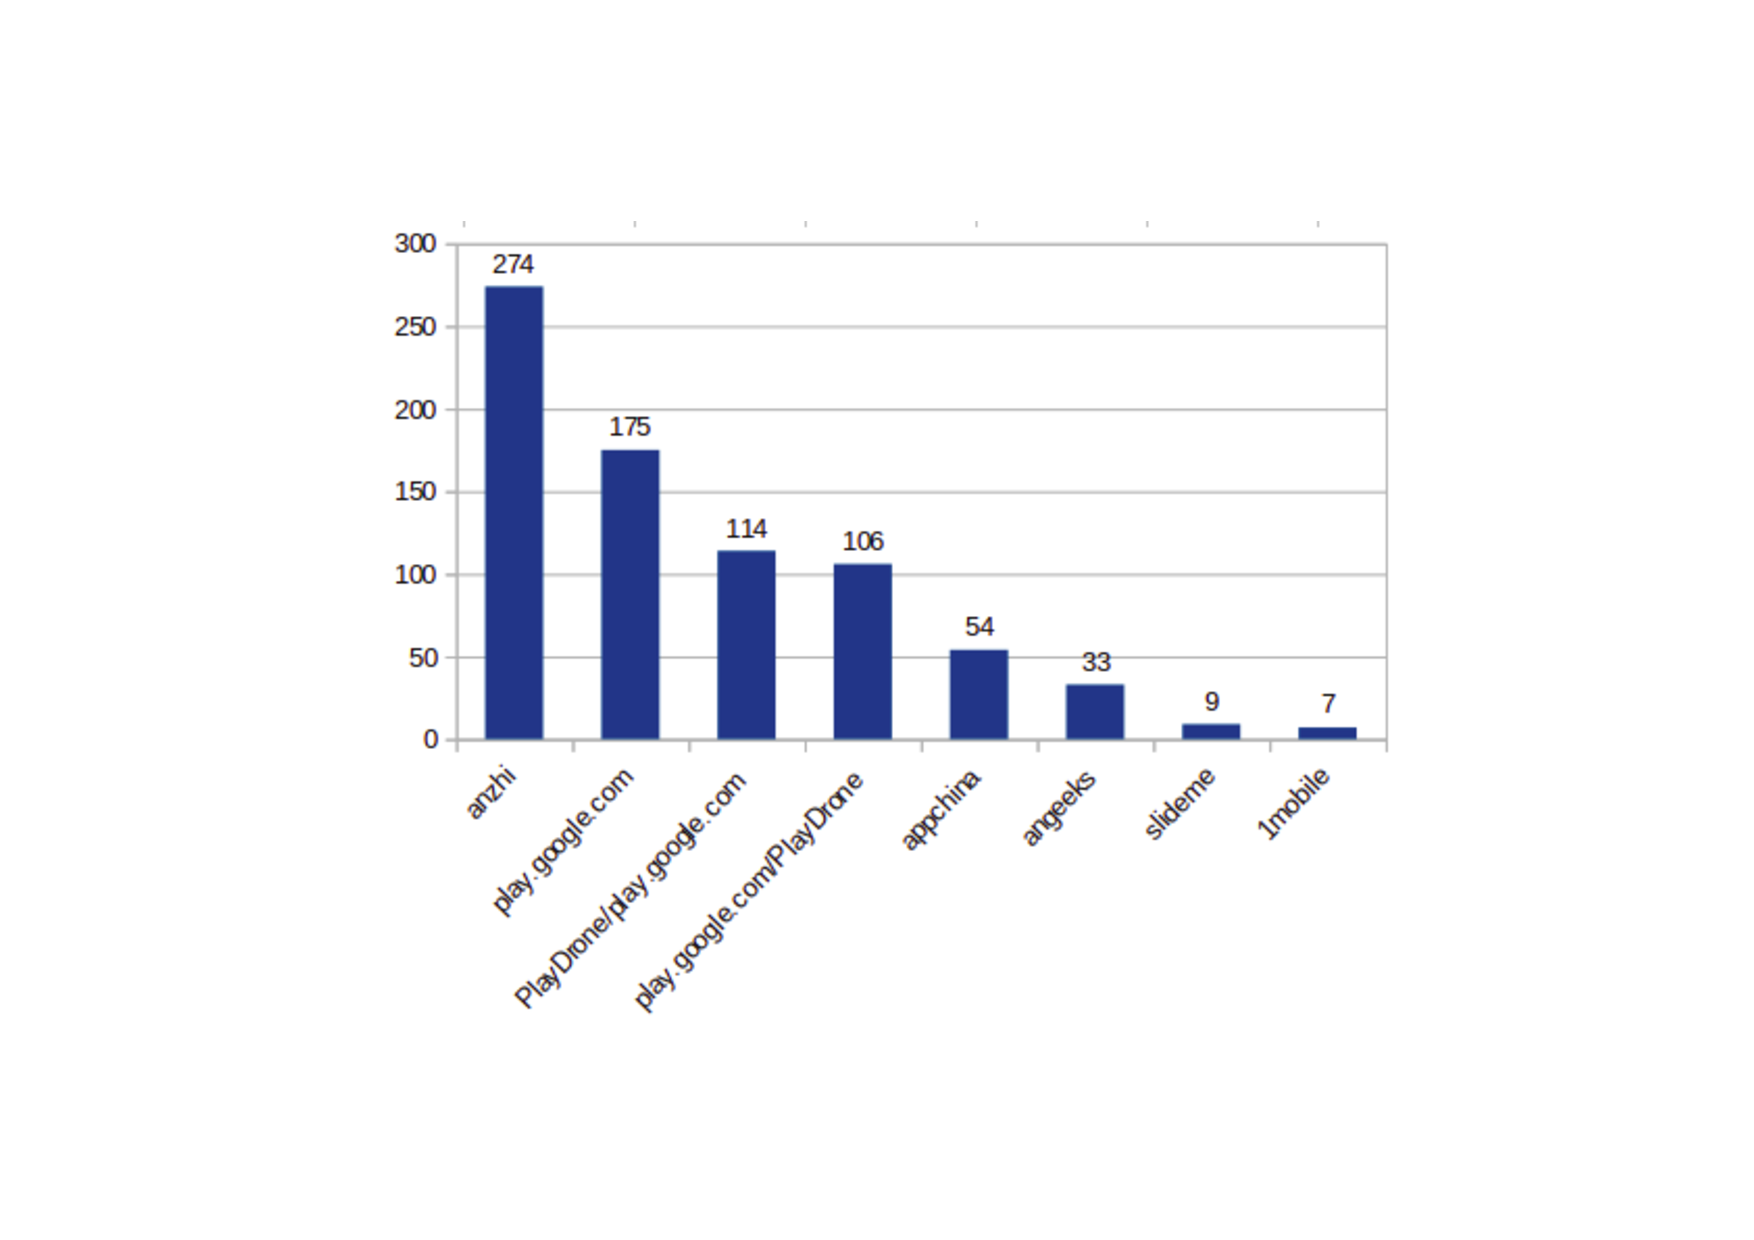
\includegraphics[scale=0.4]{images/stores.pdf}
\caption{Markets where malware was discovered.}
 \label{fig:stores}
\end{figure}

%\todo[inline]{Since the choice for DroidBot is not related to the goal of this section (Constructing the Dataset),
%  I would rather move this whole paragraph for a different place in the paper.}

%\kn{I have removed the following as it is inconsistent with our current story. We no longer perform just a study, we offer an approach. And we no longer study all four, only the top one DroidBot and built on top of it. }

%To perform an in-depth analysis of how various factors influence the quality of android sandboxes, we could have used several state of the art test generation tools like: Monkey~\cite{Monkey}, Droidmate2~\cite{DBLP:conf/kbse/BorgesHZ18}, Droidbot~\cite{DBLP:conf/icse/LiYGC17} and Humanoid~\cite{DBLP:conf/kbse/LiY0C19}. However, we considered to use just Droidbot, since several study show that it achieved better performance results when mining sensitives resources in comparison with the state of the art~\cite{DBLP:conf/wcre/BaoLL18,DBLP:journals/jss/CostaMMSSBNR22}. Its applies a depth-first strategy (DFS)~\cite{DBLP:conf/oopsla/AzimN13} to dynamically build GUI models, collecting GUI information and running process information.


%\todo[inline]{Should we call the following section Data Collection? Yes, I will change it.}

\subsection{Data Collection Procedures} \label{sec:dataCollectionProc}


\begin{comment}

\subsection{Infrastructure}\label{sec:infra}

%\kn{We currently only use one test generation tool. The following paragraph needs to be adjusted to reflect that} 
%For our study, we require an extensive infrastructure that will allow us to integrate different test case generation tools. To this end, we used and extended% DroidXP\cite{DBLP:conf/scam/CostaMCMVBC20}, a benchmark tool that allows researchers and developers, to integrate and compare test case generation tools for% mining sandboxes.

Using DroidXP, test case generation tools can be integrated and deployed easily~\footnote{The DroidXP benchmark is available at https://github.com/droidxp/benchmark}. Another reason to use DroidXP is that it relies on DROIDFAX~\cite{cai2016understanding}, which allowed us to instruments Android apps and collect important information about their execution. For example, this can be used to query for the calls to the sensitive APIs from an app during executions which is important to monitor malicious behavior. 

%\kn{I have commented out the following and shortened it as this is too verbose information about DroidXP's tooling}
The DroidXP relies on a Simple Command Line (CLI) that  provides commands for execution of different experiments with several setup, following parameters:
\newline
\newline
\textbf{DroidXP:} python main.py [-h] [--list-tools] [-tools] toolName [-t] timeSeconds [-r] repetition [--list-outputs] [--output] output [--debug] [--version]\newline
\newline
One can show help message [-h], list available test generation tools [--list-tools], test tools used in the experiment (toolName), threshold of the execution time in the experiment (timeSeconds), number of repetitions used in the experiment (repetition), list available output formats [--list-outputs], output formtat that will be used to show results (default: basic) (output),
run in DEBUG mode (default: false) [--debug] and print DroidXP version [--version].

Follow an example of a command line that executes DroidXP for three minutes (180 seconds), at test generation tools Monkey, repeating all the performance three times, and outputting the final result at a CSV file format:
\newline
\newline
\textbf{python main.py -tools monkey -t 180 -r 3 --output csv}
\newline
\end{comment}


We take advantage of the DroidXP infrastructure~\cite{DBLP:conf/scam/CostaMCMVBC20}
for data collection. DroidXP allows researchers to compare 
test case generation tools for malware identification using the
mining Android sandbox approach. Although the comparison of test
case generation tools is not the goal of this paper, DroidXP
is also useful for supporting the following steps of our study.

\begin{description}
 \item[(Step 1) Instrumentation:] In the first step,
we configure DroidXP to instrument all pairs of apps in our dataset.
Here, we instrument both versions of the apps (APK files) so that
we can collect relevant information during their execution. Under the hood, DroidXP leverages
DroidFax~\cite{DBLP:conf/icsm/CaiR17a} to instrument the apps and collect static
information about them. To improve the performance across multiple executions,
this phase executes only once for each version of the apps in our dataset.

\item[(Step 2) Execution:] In this step, DroidXP first installs the (instrumented) version of the APK files in the
  Android emulator we use in our experiment and then starts a test case generation tools for executing the app. To perform the apps executions, our study build upon DroidBot~\cite{DBLP:conf/icse/LiYGC17} which is considered the state of the art in mining sandbox approaches in terms of accuracy. To also ensure
  that each execution gets the benefit of running on a fresh Android instance without biases that could stem out of history,
  DroidXP wipes out all data stored on the emulator that has been collected from previous executions.

%\kn{Is the result analysis into logcat done by DroidXP or an extension by us? In general, it is unclear what is existing in DroidXP already and what we do. Isnt logcat a separate tool. If this is done by DroidXP, please make it clear that DroidXP invokes logcat on its own}%
\item[(Step 3) Data Collection:] During the execution, DroidXP collects all relevant information (such as calls to sensitive APIs,test coverage metrics, and so on). We use this information to understand the performance of the mining sandbox approach for malware detection. We extended DroidXP with a new component (DroidXPTrace), which allows us to investigate dynamic call graphs from the outcomes of a DroidXP execution. This was not possible using vanilla version of DroidXP %\rb{(I am note sure about this sentence)}.
%  \fh{I think that we have to separate this data collection section. One for sensitive APIs extract and other for trace extract. The 3 steps presented here must talk about just the first extract, and we must create another one for the second.  }
\end{description}

%\todo[inline]{I am not really happy with the previous structure of this section. Trying to refactor it in two sections: Data Collection Procedures and Data Analysis Procedures.}

\subsection{Data Analysis Procedures} \label{sec:dataAnalysisProc}

\subsubsection{Malware Identification} \label{sec:malwaresetup}
As described in the previous section, for malware identification we leverage DroidXP to extract information about sensitive APIs called by app at both versions (benign/malicious). As a first step, given one benign app version, our approach first collects all sensitive APIs from app code through the instrumentation step (static analysis). Then, at the execution step, we use Droidbot to collect all sensitive APIs called in the range of $3$ minutes (dynamic analysis). This second analysis is also important since it can disclose some sensitive APIs calls ignored by static analysis. Malware may use dynamic features (such as reflection) to introduce malicious behavior, which can change the behavior of classes, interfaces, methods, and fields at runtime~\cite{DBLP:journals/spe/ZhangLTX18,DBLP:journals/tosem/LiTX19}. The instrumentation step is made once, while the execution step is performed $3$ times. The result of instrumentation and all execution is finally joined forming a final set of all sensitive APIs called by app benign version. The same procedure is made at the malicious app version, and finally, we just compare the $2$ final sensitive APIs sets. The following rule is applied to decide if the analyzed APP is described as a malware:

\begin{enumerate}
    \item If the difference between the $2$ final set is an empty set, the app represents a benign app (false negative).
    \item If the difference between the $2$ final set contains at least 1 element (injected by malicious version), the app represents a malicious app (true positive).
\end{enumerate}

In additional, we also leverage from this procedure to list the sensitive APIs most injected by malicious app version at our dataset. Figure~\ref{fig:sensitiveAPI} illustrates this procedure.

%\fh{here I have to insert the figure}

\begin{figure}[ht]
\centering
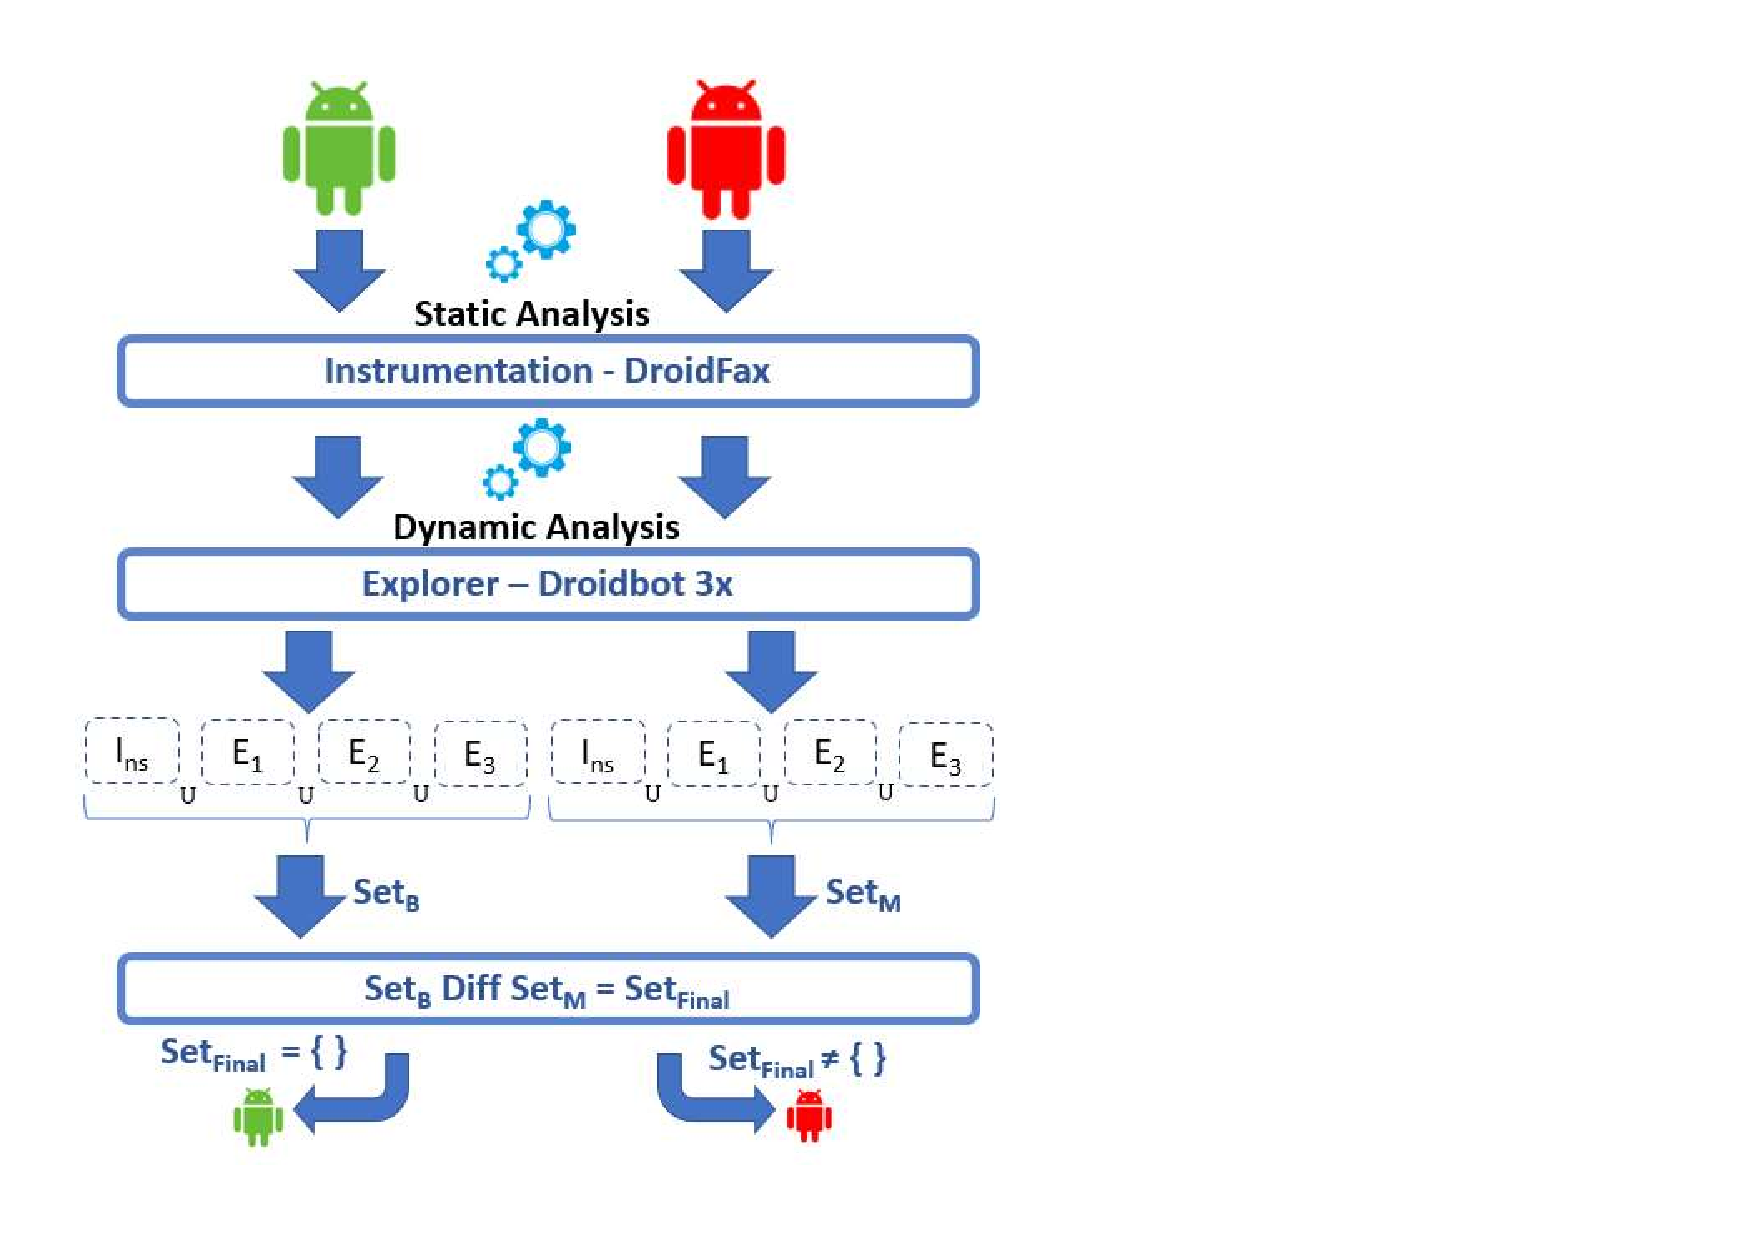
\includegraphics[scale=0.4]{images/sensitiveAPIdiff.pdf}
\caption{All procedure for malware identification using sensitive API set diff.}
 \label{fig:sensitiveAPI}
\end{figure}



%\todo[inline]{Handrick, could you please write about the malware identification procedure?}

\subsubsection{Trace Analysis} \label{sec:pathsetup}

%\todo[inline]{Handrick, is it possible to run the Trace Analysis for all apps?}

As we discussed in the previous section, we take advantage of DroidXPTrace to build the dynamic call graphs that characterize the execution of each version of the apps in our dataset. Our goal
here is to explore how many pairs of apps call the same set of sensitive APIs, though using different
traces. We conjecture that differences in the traces might be used to complement the mining sandbox
approach for malware identification. As such, here we execute the trace
analysis for all app pairs of our dataset, and check if there is the situations in which the basic version of the mining sandbox approach was not able to correctly classify the malign version of an app as a malware, however it has a different execution trace. For detecting different trace, we performed an evaluation of the dynamic call graph of each pair. Our procedure check if there is some new node, representing a new sensitive API at malicious version, or a new edge($x$, $y$), where $x$ and $y$ indicates a method $x$ calling a sensitive method $y$.

%\rb{(Not sure if this is the right decision. I do not see any problem in running
%  this study for all pairs.)}. 
%% we  investigate those app pairs that were not described as a malware during the exploratory step, i.e,
%% the test generation tool DroidBot collected the same set of sensitive APIs for both version. If a dynamic call graph
%% of these app pairs presented different traces from entry point to sensitive APIs call at both versions, we suspect this to indicate presence of malware.
Figure~\ref{fig:callGraph} illustrates an example of benign and malicious call graphs.
Although both app versions access the same set of sensitive resources, the
malicious version follows a different execution trace. 


\begin{figure}[ht]
\centering
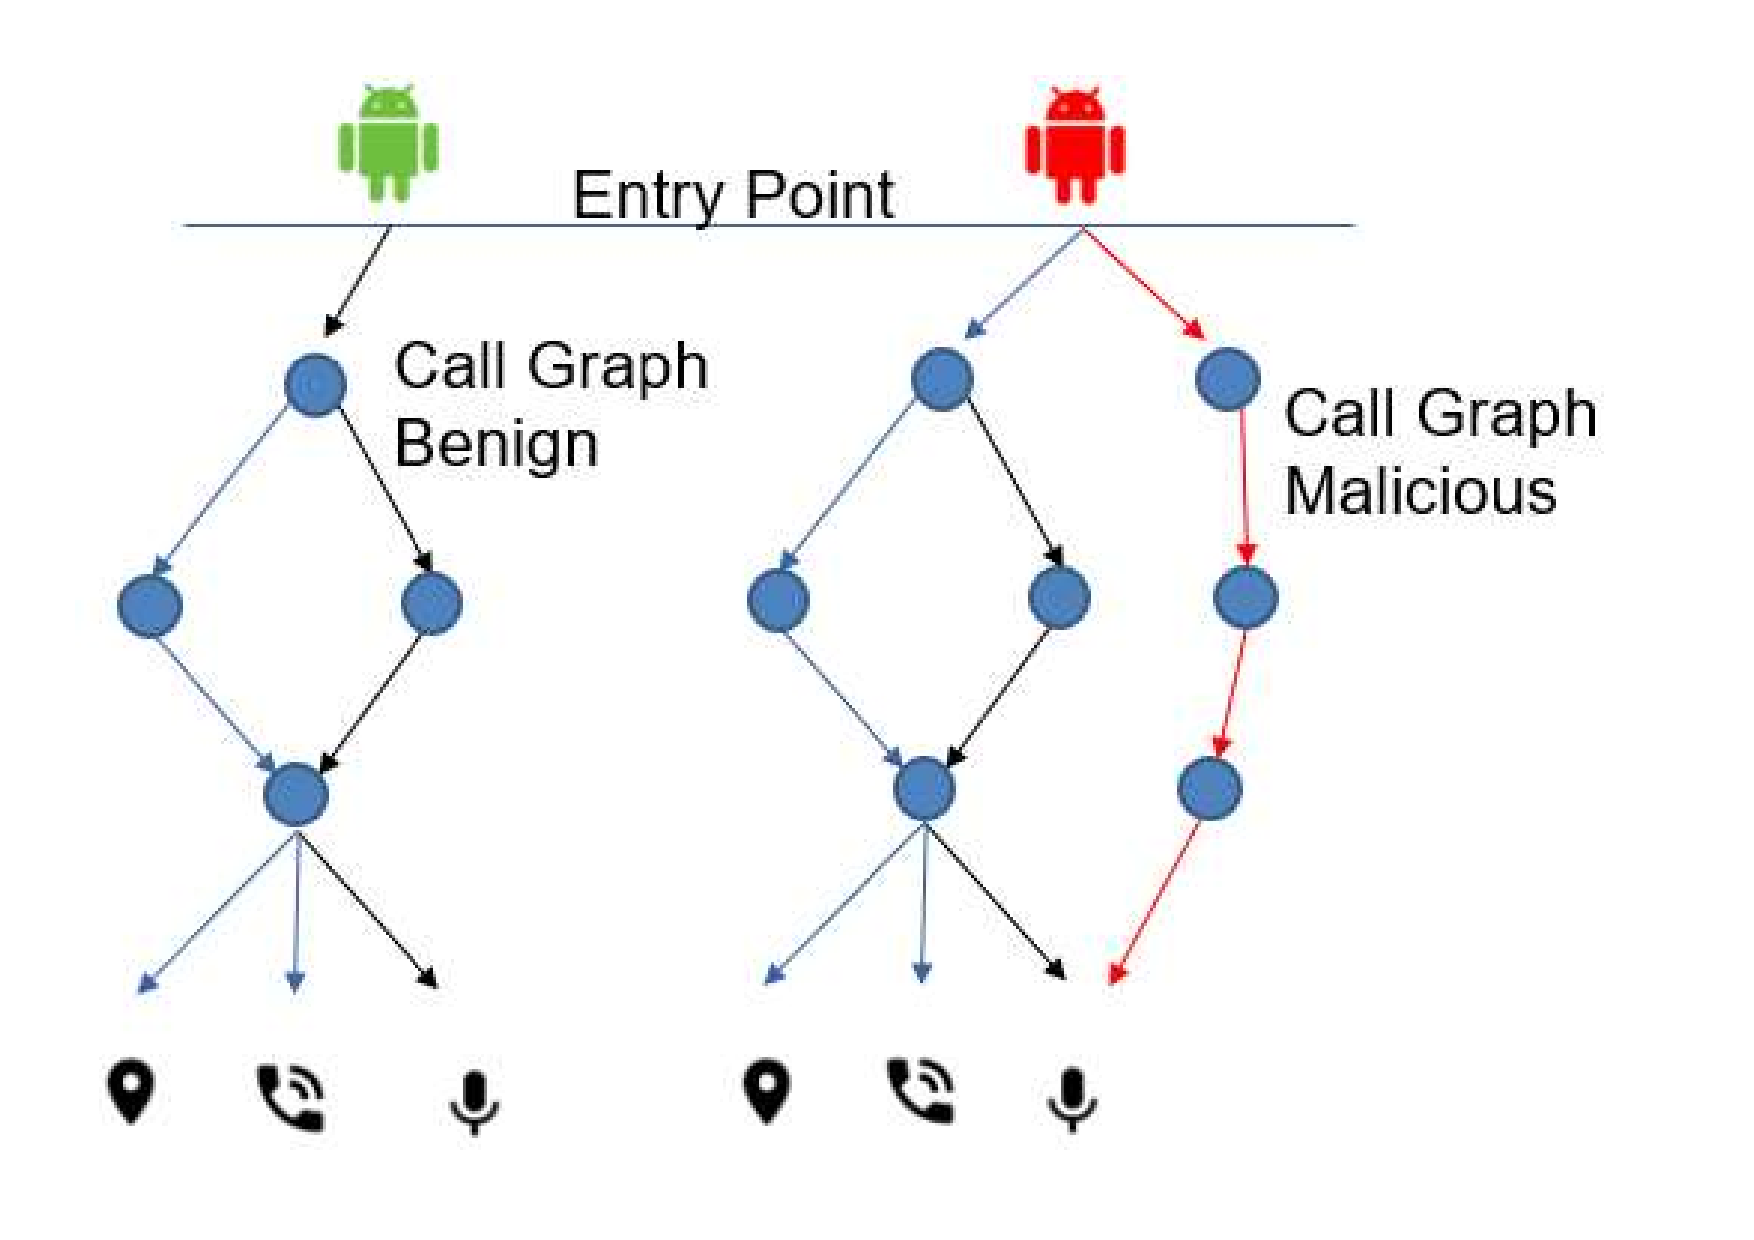
\includegraphics[scale=0.25]{images/maliciousCallGraph.pdf}
\caption{Illustrative example of the trace analysis. In this case, both versions call the same set of sensitive APIs. Nonetheless,
 the traces between the entry point and the calls to sensitive APIs diverge.}
 \label{fig:callGraph}
\end{figure}


\subsubsection{Manifest file analysis}\label{sec:manifestAnalysis}

Our work also observed the Manifest file of all app pairs. These files present essential security information which the Android system must make available before executing an app. Among other things, an Android app must specify in the Manifest file the list of necessary permissions and components . Unfortunately, Manifest files are not considered in the basic mining sandbox approach for malware detection, in spite of the fact that one can easily modify such a file and then repackage it in a malicious version of an app~\cite{DBLP:journals/corr/abs-1208-4536}. For instance, by inserting new permission requests or component capabilities (actions). Such injections can happen either manually or through automated scripts.

\todo[inline]{Looks like a naive approach. Note that, malware developers often use advanced techniques in order to hinder security experts detecting the presence of a malicious change in an app---using both static or dynamic analysis. The approach detailed here might be efficient only for poor designed malware. I am discussing this because we are seriously considering submiting this paper to a security venue. The people involved in Usenix Security are dealing with more advanced situations, like malware that changes its behavior when it detects that it is running in um emulator, for instance.}

Automated process sometimes generate Manifest file with duplicate permission requests, as the original app might already contain the permission request. Such duplication also happens when repackaged apps add a component with a capability which was requested by another component. On top of this, our manifest analysis also allows us to monitor suspicious new permissions or excessive amounts of permissions. 

To extract and analyze the Manifest file, we used an in-house Android SDK analyzer called \textit{apkanalyzer}\footnote{apkanalyzer is included in the Android SDK Tools package and provides insight into the Android app components.}. We implemented a python script that uses \textit{apkanalyzer} and computes which malicious apps had duplicated request permission or duplicated actions. The script also extracts how many permissions were requested by all apps, to help us monitor potential suspicious features. Listing~\ref{lst:androidManifestDupli} and Listing~\ref{lst:androidManifestAction} present an example of duplicated permission extracted from malicious version of the app \textbf{[com.ifeel.frogjump]}, and an example of duplicated component capabilities from malicious version of the app \textbf{[com.koushikdutta.superuser]} respectively:

%\kn{app-8 according to what table? reference please}. 

\begin{lstlisting}[caption={Example of duplicated permission from malicious version of app (com.ifeel.frogjump)}, language=Java,
    basicstyle=\fontsize{6}{5}\selectfont\ttfamily,
    label={lst:androidManifestDupli}]

13:M >  <uses-permission
        android:name="android.permission.READ_PHONE_STATE" />

16:M >  <uses-permission
        android:name="android.permission.ACCESS_COARSE_LOCATION" />

19:M >  <uses-permission
        android:name="android.permission.INTERNET" />

22:M >  <uses-permission
        android:name="android.permission.ACCESS_NETWORK_STATE" />
    .
    .
    .
134:M > <uses-permission
        android:name="android.permission.INTERNET" />

137:M > <uses-permission
        android:name="android.permission.WAKE_LOCK" />

140:M > <uses-permission
        android:name="android.permission.READ_PHONE_STATE" />

143:M > <uses-permission
        android:name="android.permission.ACCESS_NETWORK_STATE" />

146:M > <uses-permission
        android:name="android.permission.WRITE_EXTERNAL_STORAGE" />

149:M > <uses-permission
        android:name="android.permission.ACCESS_WIFI_STATE" />
\end{lstlisting}

\begin{lstlisting}[caption={An example of duplicated component capability from malicious version of app (com.koushikdutta.superuser)}, language=Java,
    basicstyle=\fontsize{6}{5}\selectfont\ttfamily,
    label={lst:androidManifestAction}]

101:M > <receiver
102:M >  android:name=".SuCheckerReceiver">
103:M >  <intent-filter>
104:M >    <action
105:M >      android:name="android.intent.action.BOOT_COMPLETED" />                 
106:M >  </intent-filter>
107:M > </receiver>
108:M > <receiver
109:M >  android:name=".PackageChangeReceiver">
110:M >  <intent-filter>
111:M >    <action
112:M >      android:name="android.intent.action.BOOT_COMPLETED" />
113:M >    <data
114:M >      android:scheme="package" />
115:M > </intent-filter>
     .
     .
     .
\end{lstlisting}

Listing~\ref{lst:androidManifestDupli} suggests that the four first requested permission could have been added automatically. Listing~\ref{lst:androidManifestAction} presents a duplicated component that might also suggest that the first was newly injected by a naive hacking script.


%% We extended DroidXP with a new component (DroidXPTrace) that allows us to build a dynamic call graph from the outcomes of a DroidXP execution. This was not possible using vanilla version of DroidXP \rb{(I am note sure about this sentence)}. DroidXPTrace, using the result from Phase 3 of DroidXP, creates a call graph of app pair, exploring traces from its entry point to sensitive API access. In the end, it compares both call graphs (benign and malicious app version), and generated a JSON file recording the following information:
%\kn{I have rephrased the previous paragraph, please check if it is still accurate}. 

%\kn{Overall the following bits in the rest of this subsection are a bit confusing.  You use the word trace and graph interchangeably. is it a graph or a trace. And finally the connection to paths taken comes out of nowhere. I propose rephrasing this part with an example data from some app. Only one of the columns is enough. Even if the example is an artificial one it is fine. Important is that it becomes clear what data is recorded. }
%% \begin{itemize}
%% \item \texttt{benign}: Name of log file from the benign app version
%% \item \texttt{malign}: Name of log file from the malicious app version
%% \item \texttt{benignGraphs}: call graphs that contain traces with access to sensitive methods in the benign version of the app.
%% \item \texttt{malignGraphs}: call graphs that contain traces with access to sensitive methods in the malicious version of the app.
%% \item \texttt{methodsAccessedOnlyByMalign}: The sensitive methods that are accessed only by the malicious version of the app. This information is important to identify if a particular sensitive call that is undetected by a sandbox occurs only in a malicious version.
%% \item \texttt{benignGraphContainsMalignGraph}: Comparison between benign and malicious sub-callgraphs
%% \item \texttt{hasDifferentTraces}: whether the benign and malicious app version have different traces to sensitive resources. 
%% \end{itemize}

%%  This information helped us to explore traces between an app's entry point and its access to sensitive methods during run time.
%%  \kn{What I have commented below is talking about the study itself and not the setup. Please ensure other such instances are removed if I have missed them.}
%%  %This investigation shows that in several situations, although both app versions (benign-malicious) access the same set of sensitive resources, they access them using different traces, which could mean malicious sensitive resource access.





\subsection{Execution Settings}\label{sec:hardware}

We deployed our experiment on a 32-Core, AMD EPYC 7542 CPU, 512 GB RAM, storage Samsung SSD 970 EVO 1TB machine running a 64-bit Debian  GNU/Linux 11. We also configured our emulator to run all selected apps on Google Android version 9.0, API 28, 512M SD Card, 7GB internal storage, with X86 ABI image.

For our study, we configured DroidXP to run each of the $800$ app pairs using Droidbot for three minutes. To mitigate noise, we repeated the full process three times which took in total ($800 \times 2$ apps (benign/malicious) $\times 3$ runs $\times 3$ min) + ($800 \times 2$ apps $\times 1.5$ min for emulator reboot) $\apeq 240$ machine hours.
%\kn{This number needs to be changed here too. I suggest introducing a macro for this and using it everywhere to make sure everytime our experiment evolves, we don't need to change this everywhere} 

%\kn{Initial? Was there a follow up study, if not please use only study. This is feedback for all instances with the word initial}

Although it was possible to run more than 10 emulators in parallel on one physical machine, to avoid any interference resulting from context switching within the operating system, we chose to run one emulator at a time. Hence, all evaluation processes took around $12$ days and additional $5$ days for environment configuration.

% In the following subsections, we describe the setup required to perform custom analysis that were central to our study.

%% \subsection{Sensitive API setup} \label{sec:sensitivapi}
%% \fh{Here the text talk about false positive. We have to change to talk about how we extract the most sensitive APIs used by malicous apps }
%% \kn{I am ignoring this subsection for review as it is no longer relevant. Please add some details about the sensitive APIs collection so it can be extended upon.}
%% To perform the false positive analysis we used the infrastructure of DroidXP, described in section~\ref{sec:infra}. After finishing \textbf{Phase 2 (execution)}, we have all explorer information about the apps under analysis by Droidbot test generation tools.

%% Our analysis concert just at the benign version of apps, since false positive alarm could occur when some expected behavior from the benign app version is not seen during mining step. Hence, as a first step we collect all sensitive methods (SM) by the union of three execution of mine sandbox at all benign apps version. With this step, we could have a base set of sensitive methods called by each benign version from all 95 apps explored in our study. After, we executed mine sandbox again at the same set of benign apps version seven times. At each execution we observed the set of sensitive methods called, and compare them with the initial set of sensitive methods composed by the union of methods explored by the first three executions. In the end, we executed 7 tests, checking if the difference between all the these sets are empty sets, as below:\newline

%% \begin{enumerate}[(Test 1)]
%%  \item {$\left\{\left\{SM01\right\} \cup \left\{SM02\right\} \cup \left\{SM03\right\}\right\} \textit{diff} \left\{SM04\right\} = \emptyset$}
%%  \item {$\left\{\left\{SM01\right\} \cup \left\{SM02\right\} \cup \left\{SM03\right\}\right\} \textit{diff} \left\{SM05\right\} = \emptyset$}
%%  \item {$\left\{\left\{SM01\right\} \cup \left\{SM02\right\} \cup \left\{SM03\right\}\right\} \textit{diff} \left\{SM06\right\} = \emptyset$}
%%  \item {$\left\{\left\{SM01\right\} \cup \left\{SM02\right\} \cup \left\{SM03\right\}\right\} \textit{diff} \left\{SM07\right\} = \emptyset$}
%%  \item {$\left\{\left\{SM01\right\} \cup \left\{SM02\right\} \cup \left\{SM03\right\}\right\} \textit{diff} \left\{SM08\right\} = \emptyset$}
%%  \item {$\left\{\left\{SM01\right\} \cup \left\{SM02\right\} \cup \left\{SM03\right\}\right\} \textit{diff} \left\{SM09\right\} = \emptyset$}
%%  \item {$\left\{\left\{SM01\right\} \cup \left\{SM02\right\} \cup \left\{SM03\right\}\right\} \textit{diff} \left\{SM10\right\} = \emptyset$}
 
%% \end{enumerate}

%% We observed if all execution explored the same sensitive methods at each benign app in our dataset (95 app pairs). We consider that occur a false positive alert when at least one of seven tests fail, i.e. if one of the 7 tests returns a non-empty set.

%% As a second step, we also choose a random execution, and check if the set of sensitive methods collected by this execution, is the same of other 9 sensitive methods set, collected by others 9 executions. At this second step, the fifth execution was the choose one as a base execution for tests, as described below:\newline

%% \begin{enumerate}[(Test 1)] \setcounter{enumi}{7}
%%  \item {$\left\{SM05\right\} \textit{diff} \left\{SM01\right\} = \emptyset$}
%%  \item {$\left\{SM05\right\} \textit{diff} \left\{SM02\right\} = \emptyset$}
%%  \item {$\left\{SM05\right\} \textit{diff} \left\{SM03\right\} = \emptyset$}
%%  \item {$\left\{SM05\right\} \textit{diff} \left\{SM04\right\} = \emptyset$}
%%  \item {$\left\{SM05\right\} \textit{diff} \left\{SM06\right\} = \emptyset$}
%%  \item {$\left\{SM05\right\} \textit{diff} \left\{SM07\right\} = \emptyset$}
%%  \item {$\left\{SM05\right\} \textit{diff} \left\{SM08\right\} = \emptyset$}
%%  \item {$\left\{SM05\right\} \textit{diff} \left\{SM09\right\} = \emptyset$}
%%  \item {$\left\{SM05\right\} \textit{diff} \left\{SM09\right\} = \emptyset$}
%% \end{enumerate}

%% As the first analysis, we also consider a false negative occurrence, if one of the 9 remaining tests returns a non-empty set.

